\section{Closed-Loop Simulation Environment} \label{closed-loop-sim-env}%\label{s:overview}

% say we are addressing RQ 1 in the beginning

RocketPy is inherently a continuous-time simulator as it integrates a set of differential equations to propagate the rocket's trajectory. However, its implementation exposes a unique callback interface described in Section \ref{background-rocketpy}. While not designed for co-simulation, it can be repurposed as a synchronisation point that exchanges state with an external component at each discrete step. This is one of the key observations that drives this study, as it paves the way for coupling RocketPy with flight software in a closed-loop configuration.

In this study, the F Prime flight software is configured to perform three control tasks: deploying air brakes during the coasting phase to reach a target apogee of 3000\,m, triggering the drogue parachute at apogee and deploying the main parachute during descent. 

The following sections describe the simulation environment. Section~\ref{framework-arch} provides an overview of the architecture, introducing the three modules of the framework and the communication layer among them. Section \ref{s:fsw-arch} presents the flight software architecture, while Sections~\ref{lockstep}, \ref{snapshot}, and \ref{rate-group} detail each of the three coupling architectures evaluated in this study. Collectively, these sections answer RQ1 by documenting design and implementation decisions that support a closed-loop simulation environment involving RocketPy and F Prime.

\subsection{Framework Architecture}\label{framework-arch}
The framework proposed in Figure \ref{fig:architecture-diagram} places an Orchestrator between RocketPy and the F Prime FSW, a decision motivated by co-simulation literature of a coordinating component driving the exchange between simulators~\cite{gomes2017cosimulation}. Unlike a typical co-simulation coordinator, however, this Orchestrator does not control simulated time progression. RocketPy, instead, owns the simulation time internally via its integrator, while the Orchestrator is only invoked when RocketPy reaches a scheduled controller callback, set to 10Hz. To force the integrator to stop exactly at each scheduled node rather than stepping past it, \texttt{time\_overshoot} is disabled. RocketPy exposes four separate timing parameters relevant to this framework: the controller callback sampling rate described above, the sampling rate of RocketPy's built-in sensor models (accelerometer, barometer, gyroscope), the sampling rate of the drogue and main callback functions, and the solver's internal integration time step (\texttt{min\_time\_step} and \texttt{max\_time\_step}). These can, in principle, be set independently of one another.

Retaining the Orchestrator as a mediator, despite its non-compliance with strict co-simulation, offers two practical advantages. First, it decouples the interface from both the simulator and the flight software, meaning that either could be replaced without changes to the other. Second, it provides a natural point at which to apply additional processing, such as fault injection, before the sensor data is forwarded to the flight software.

To support fault injection, the Orchestrator includes a \texttt{FaultInjector} module that intercepts sensor data before it is forwarded to the FSW. This module has the opportunity to inject several faults to the outgoing sensor packets. In this study, a single fault is evaluated: a barometric freeze, where the barometric pressure reading is captured and held constant for all following packets. This allows failure-recovery behaviour to be tested within the same closed-loop configuration, without modifications to either RocketPy or the flight software.

\begin{figure}[h]
    \centering
    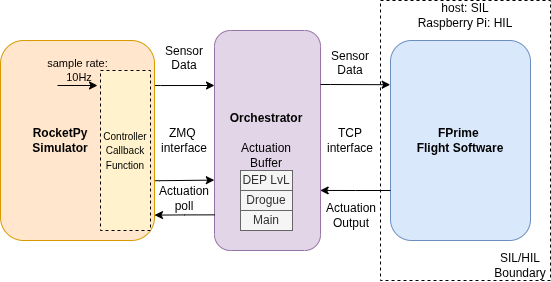
\includegraphics[width=0.5\textwidth]{figures/arch.png}
    \caption{The simulation architecture, consisting of the RocketPy simulator, the Orchestrator and the F Prime flight software.}
    \label{fig:architecture-diagram}
\end{figure}

\subsubsection{Communication Layer}
ZMQ was selected as the communication layer between RocketPy and the Orchestrator for two reasons. First, it is language agnostic, allowing the orchestrator interface to be used with simulators written in languages other than Python. Second, when both processes run on the same machine, ZMQ communicates via shared memory rather than the network stack, minimising communication overhead in SIL configurations. On the F Prime side, TCP was chosen over UDP for two reasons. First, one of the coupling strategies evaluated (Lockstep, introduced in Section \ref{lockstep}) requires reliable and ordered delivery. Second, the same deployment communicates over the local loopback interface in SIL and over a physical Ethernet link in HIL with no changes required to the communication layer. The trade-off is that TCP introduces connection overhead that UDP would avoid. 

\subsubsection{Sensor Data Flow}
In each controller callback function, RocketPy-simulated sensor readings are passed to the Orchestrator via ZMQ. Sensor data consists of accelerometer, gyroscope, and barometer readings, taken from RocketPy's sensor models along with the current simulation time $t$. The Orchestrator then forwards these readings directly to F Prime over TCP, where they are received by the flight software as if received from physical sensors.


\subsubsection{Actuation Data Flow}

The return path is more constrained. RocketPy's controller callback expects a synchronous return value, as there is no mechanism to send a control command to the simulation while it is running. The Orchestrator, therefore, maintains a buffer of the last known actuation output received from F Prime, consisting of the air brake deployment level, a continuous value in the range $[0,1]$ and two boolean deployment flags for the drogue and main parachutes. How the Orchestrator uses this buffer at callback time depends on the coupling strategy, as described in Sections~\ref{lockstep} -- \ref{rate-group}.


\subsubsection{SIL/HIL Capabilities}
The framework supports SIL and HIL execution without changes to Orchestrator or RocketPy. In SIL, F Prime runs as a native process on the same host machine, with TCP communication over the local loopback interface. In HIL, the same F Prime deployment is cross-compiled for the Raspberry Pi, with TCP communication routed over a physical Ethernet Link. The only change required is pointing the Orchestrator at the FSW's IP and port. A second capability comes from F Prime's topology abstraction. Since a topology is just a declarative wiring of components, different topologies can be defined for different flight computer architectures without changing the underlying framework. This same abstraction also supports separate topologies for simulation and for actual flight. For instance, both topologies would share the same logic components but swap out the sensor components, where the flight topology reads from physical sensors, while the simulation topology reads from the Orchestrator via the same interface.



\subsection{Flight Software Architecture}\label{s:fsw-arch}
The fidelity of the SIL and HIL configurations depends on the flight software as much as on the simulation infrastructure. The deployment architected in this study mirrors a real avionics system, replacing only the hardware drivers with simulated counterparts.

\begin{figure}[h]
    \centering
    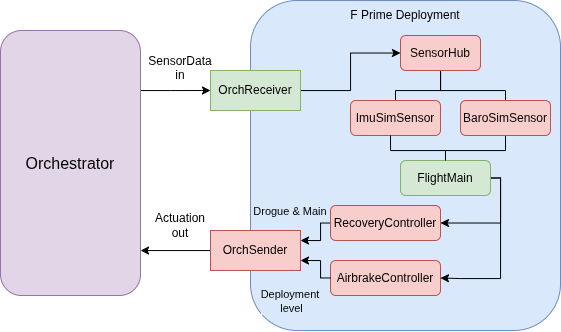
\includegraphics[width=0.5\textwidth]{figures/fsw-arch.png}
\caption{General FSW architecture. Components are coloured 
by execution type: green for active, red for passive.}
    \label{fig:fsw_architecture-diagram}
\end{figure}

The proposed FSW architecture is illustrated in Figure~\ref{fig:fsw_architecture-diagram}. Component colours indicate execution type specific to F Prime: green for active, red for passive. Communication with the Orchestrator is handled by two dedicated components: \texttt{OrchReceiver}, a TCP client that receives incoming sensor data, and \texttt{OrchSender}, a TCP server that transmits actuation outputs back to the Orchestrator. 

Incoming sensor data is distributed via the \texttt{SensorHub}. This component holds the data packet as it arrives from the Orchestrator, including the simulation time $t$. The \texttt{SensorHub} distributes sensor data to its respective sim sensor components, \texttt{ImuSimSensor} and \texttt{BaroSimSensor}, which repackage accelerometer/gyroscope and barometer readings into the port types expected by the flight logic. This abstraction mirrors real flight software, where \texttt{FlightMain} reads from the same sensor interfaces regardless of whether the source is simulated or physical hardware. These SimSensors are present in the Figure but are only active in the clock-driven topology, as described in Section~\ref{fsw-exec-topologies}.


\texttt{FlightMain} is the central flight logic component. It is responsible for phase detection and sending control outputs. It delegates air brake control to \texttt{AirbrakeController}, which computes the deployment level during the coasting phase, and to \texttt{RecoveryController} for parachute deployment actuations.


\subsubsection{FSW Execution Topologies} \label{fsw-exec-topologies}
During the implementation of the flight software, two execution topologies emerged as fitting for the coupling strategies under evaluation. This split reflects a long-standing distinction in real-time systems between time-triggered and event-triggered architectures~\cite{scheler-time-trigger-event-trigger}. In a time-triggered system, activities are executed periodically at predetermined points regardless of external events. In contrast, in an event-triggered system, execution is initiated directly by the occurrence of a signal or event. In this study, the clock-driven topology corresponds to the time-triggered model, while the sensor-driven topology corresponds to the event-triggered model. Both are illustrated in Figures~\ref{fig:clock-driven-arch-diagram} and~\ref{fig:sensor-driven-arch-diagram}. The choice of topology for a given coupling strategy is described in Sections~\ref{lockstep}--\ref{rate-group}.


The clock-driven topology illustrated in Figure \ref{fig:clock-driven-arch-diagram} decouples data arrival from FSW execution. \texttt{OrchReceiver} runs on its own thread, continuously receiving sensor packets and updating \texttt{ImuSimSensor} and \texttt{BaroSimSensor} buffers via the \texttt{SensorHub}. \texttt{FlightMain} is driven independently by a \texttt{LinuxTimer}, which ticks a passive \texttt{RateGroupDriver} at a configurable frequency. On each tick, \texttt{FlightMain} polls the latest available values from these buffers, regardless of when the last packet arrived. This topology mirrors real flight software more closely, where the avionics loop runs on a fixed schedule driven by a hardware timer, and sensor reads are decoupled from the arrival of new data.

\begin{figure}[h]
    \centering
    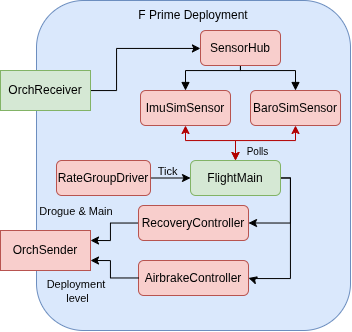
\includegraphics[width=0.4\textwidth]{figures/rate-group-arch.png}
   \caption{The clock-driven topology. \texttt{FlightMain} 
is driven by a \texttt{LinuxTimer} at a configurable frequency, reading sensor data from the SimSensor buffers on each tick.}
    \label{fig:clock-driven-arch-diagram}
\end{figure}

The sensor-driven topology, illustrated in Figure~\ref{fig:sensor-driven-arch-diagram}, removes this decoupling. Both \texttt{OrchReceiver}  and \texttt{FlightMain} are active components, each running on its own thread. \texttt{OrchReceiver} continuously listens for incoming sensor packets and, upon receipt, forwards them to \texttt{SensorHub}, which passes the data packet directly to \texttt{FlightMain}'s message queue. Unlike clock-driven topology, \texttt{ImuSimSensor} and \texttt{BaroSimSensor} are absent, as the incoming sensor packet is itself the tick that drives \texttt{FlightMain}, so there is no intermediate state to hold. This makes the execution order deterministic with respect to sensor arrival, since \texttt{FlightMain} always processes each packet directly rather than polling a buffer that may or may not have been updated since the last tick.



\begin{figure}[h]
    \centering
    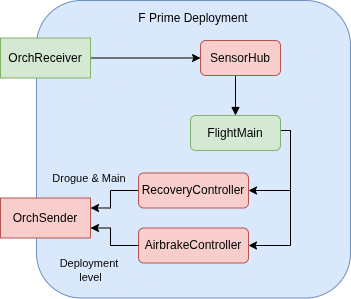
\includegraphics[width=0.4\textwidth]{figures/sensor-driven-arch.png}
    \caption{The sensor-driven topology, in which \texttt{OrchReceiver} triggers \texttt{FlightMain} directly on each incoming sensor packet.}
    \label{fig:sensor-driven-arch-diagram}
\end{figure}

\subsubsection{Flight Logic} \label{flight-logic}
The flight software implements two independent controllers invoked from \texttt{FlightMain}: \texttt{AirbrakeController}, which manages drag control during the coasting phase via a PI controller, and \texttt{RecoveryController}, which handles parachute deployment via apogee detection.

\texttt{AirbrakeController} activates after motor burnout. Burnout is detected when the vertical acceleration from the IMU drops below 15 $m/s^2$ following a period of sustained positive thrust. During the coasting phase, the controller estimates the predicted apogee as follows:

\begin{equation}
\hat{a} = h + \frac{v_z^2}{2g}
\end{equation}

\noindent where $g = 9.81\,\text{m/s}^2$, $v_z$ is the vertical velocity integrated from IMU acceleration readings, and $h$ is the barometric altitude derived from the International Standard Atmosphere model:

\begin{equation}
    h = 44330 \left(1 - \left(\frac{P}{P_0}\right)^{\frac{1}{5.255}}\right)
    \label{eq:baro}
\end{equation}

\noindent where $P$ is the current barometric pressure and $P_0$ is the reference pressure at the ground level that is recorded from the first reading of the flight software at initialisation.

A PI controller commands the airbrake deployment. The proportional term responds to the difference between $\hat{a}$ and the target apogee 3000~m, whereas the integral term accumulates this error over time. The air brake deployment level is clamped to $[0, 1]$ as required by RocketPy, and an anti-wind-up clamp bounds the integral term to prevent integrator saturation during extended coasting. The controller deactivates once 10 consecutive barometric readings indicate a decreasing altitude, at which point the air brakes are fully retracted. The controller constants were selected to produce stable, non-oscillatory actuation toward the 3000\,m target. Formal tuning is outside the scope of this study.

\texttt{RecoveryController} detects apogee using barometric pressure. Multiple apogee detection approaches exist, including IMU-based velocity integration and Kalman filters \cite{kimani2022detection}. Barometric detection was chosen for its simplicity, as flight logic implementation is not the focus of this study. The implementation tracks the minimum observed pressure and fires the drogue parachute only after 10 consecutive readings exceed that minimum by 0.5 hPa. The main parachute is deployed when the pressure has increased by 40 hPa above the recorded apogee minimum, corresponding to a descent of approximately 330 m under the ISA model.

The \texttt{RecoveryController} component facilitates the testing of failure-recovery behaviour by implementing fallback logic for cases where barometric readings are not reliable. If consecutive barometer readings become stale, differing by less than \texttt{BARO\_FREEZE\_DELTA} for \texttt{BARO\_FREEZE\_COUNT} samples after launch, the controller detects a sensor fault and switches to IMU-based apogee detection. The drogue deployment is then activated when the magnitude of the vertical IMU acceleration drops below \texttt{ACCEL\_FREEFALL\_THRESH}, indicating that the rocket has entered free fall. If the fault persists after drogue deployment, the main parachute is deployed after a fixed timeout of \texttt{MAIN\_DEPLOY\_TIMEOUT} rather than waiting for the pressure-based threshold. The constants governing both controllers are summarised in Table~\ref{tab:controller-constants}.


\begin{table}[h]
\centering

\small
\begin{tabular}{llp{3.8cm}}
\toprule
\textbf{Constant} & \textbf{Value} & \textbf{Description} \\
\midrule
\texttt{TARGET\_APOGEE}            & 3000\,m        & PI target \\
\texttt{Kp}                        & 0.001          & Proportional gain \\
\texttt{Ki}                        & 0.0001         & Integral gain \\
\texttt{INTEGRAL\_CLAMP}           & 1000           & Anti-windup bound \\
\texttt{BOOST\_ACCEL\_THRESHOLD}   & 15\,m/s$^2$    & Burnout threshold \\
\texttt{DESCENT\_COUNT\_THRESHOLD} & 10             & Descent readings to retract \\
\texttt{APOGEE\_BARO\_DELTA}       & 0.5\,hPa       & Pressure rise per confirmation \\
\texttt{APOGEE\_CONFIRM\_COUNT}    & 10              & Confirmations before drogue \\
\texttt{MAIN\_DEPLOY\_DELTA\_HPA}  & 40\,hPa        & Pressure rise for main deployment \\
\texttt{BARO\_FREEZE\_DELTA}       & 1\,hPa         & Max variation for freeze detection \\
\texttt{BARO\_FREEZE\_COUNT}       & 15             & Frozen samples before fault \\
\texttt{LAUNCH\_ACCEL\_THRESH}     & 20\,m/s$^2$    & Launch detection threshold \\
\texttt{ACCEL\_FREEFALL\_THRESH}   & 2\,m/s$^2$     & Free-fall detection threshold \\
\texttt{MAIN\_DEPLOY\_TIMEOUT}     & 20\,s          & Fallback main deploy timeout \\
\bottomrule
\end{tabular}
\caption{Constants for \texttt{AirbrakeController} and \texttt{RecoveryController}.}
\label{tab:controller-constants}
\end{table}

\subsection{Lockstep Strategy } \label{lockstep}
The Lockstep Strategy is the most tightly synchronised of the three coupling architectures evaluated in this study. It uses the sensor-driven topology described in Section~\ref{fsw-exec-topologies}. After sending the sensor data to the FSW, the Orchestrator blocks on the TCP connection, waiting for an actuation response before returning from the callback. This guarantees that every simulation step is computed using the actuation output corresponding to that exact sensor reading, meaning there is no lag between the plant model and the control output. This makes Lockstep the appropriate choice when the goal is to isolate the correctness of the flight logic itself, since eliminating timing effects removes any ambiguity between a logic error and one of execution timing.



% The cost is wall-clock time, as the simulation idles at every callback until the flight software responds.

\subsection{Snapshot Strategy}\label{snapshot}
The Snapshot strategy relaxes the synchronisation constraint of Lockstep. It also uses the sensor-driven topology, but the Orchestrator does not block after sending the sensor packet. Instead, it immediately returns the latest values in the Actuation Buffer to RocketPy and continues. \texttt{FlightMain} still processes each sensor packet, but its actuation response updates the buffer only after RocketPy has already advanced to the next step, which means that the simulation continues using the actuation from the previous tick. This reduces wall-clock time by eliminating the blocking wait, at the cost of a looser coupling between the plant state and the control output.

\subsection{Rate Group Strategy}\label{rate-group}
The Rate Group Strategy completely decouples flight software execution from the RocketPy callback. It uses the clock-driven topology, where \texttt{FlightMain} runs on a fixed hardware timer, independent of when the callback fires. The Orchestrator behaves identically to Snapshot, forwarding sensor packets and returning the latest actuation buffer value without blocking. The actuation buffer reflects whatever the FSW last computed, which may have been on a different tick from the current callback. This is the closest of the three strategies to real flight software behaviour, where the FSW loop runs on a hardware-driven schedule, independent of any external synchronisation. The trade-off is timing non-determinism, since the FSW and RocketPy run on independent clocks, the values in the actuation buffer at any given callback may have been computed on a different tick, introducing variability in control output timing. This same non-determinism makes the Rate Group strategy the hardest of the three strategies to use for isolating flight logic errors.

Together, the three strategies span a spectrum from fully synchronised to fully decoupled and are evaluated experimentally in Section \ref{experiment-design}.




% \TODO{
% This section provides a high-level outline of the proposed system or solution.
% It typically illustrates the system architecture or the interactions between the
% different solution components (via a ``boxes-and-arrows'' diagram) from a user’s
% perspective.
% }


